% 五号字体,开明式标点处理,不设置默认字体
\documentclass[UTF8, 12pt, punct=kaiming, fontset=none]{article}
\usepackage[UTF8]{ctex}
\usepackage{fontspec}
\usepackage{float}
\usepackage{graphicx}
\usepackage{subcaption}
\usepackage{pgf-umlsd}
% 品红色链接和注释
% \usepackage[colorlinks=true, linkcolor=magenta, citecolor=magenta, urlcolor=magenta]{hyperref}
% 黑色链接和注释
\usepackage[colorlinks=true, linkcolor=black, citecolor=black, urlcolor=black]{hyperref}
\usepackage{geometry}
\usepackage{fancyhdr}
\usepackage{caption}
\usepackage{framed}
\usepackage{titlesec}
\usepackage{ragged2e}
\usepackage{url}
\usepackage{cite}
\usepackage{bookmark}

\graphicspath{{figures/}}

% 字体
\IfFontExistsTF{Source Han Serif SC}
{
    \setCJKmainfont{Source Han Serif SC}
}
{
    % GitHub Actions
    \setCJKmainfont[
        Path=. ./fonts/ ,    
        Extension = . otf ,
        UprightFont = *-Regular ,
        BoldFont = *-Bold
    ]{SourceHanSerifSC}
}
\IfFontExistsTF{Source Han Sans SC}
{
    \setCJKsansfont{Source Han Sans SC}
}
{
    % GitHub Actions
    \setCJKsansfont[
        Path=. ./fonts/ ,    
        Extension = . otf ,
        UprightFont = *-Regular ,
        BoldFont = *-Bold
    ]{SourceHanSerifSC}
}
\IfFontExistsTF{DejaVu Sans}
{
    \newfontfamily\ds{DejaVu Sans}
}
{
    % GitHub Actions
    \newfontfamily\ds[
        Path=. ./fonts/ ,    
        Extension = . ttf ,
        BoldFont = *-Bold ,
        ItalicFont = *-Oblique ,
        BoldItalicFont = *-BoldOblique
    ]{DejaVuSans}
}
%\newfontfamily\cm{CMU}

% 图表标题字体
\DeclareCaptionFont{captionfont}{\ds}
\captionsetup[table]{font=captionfont}
\captionsetup[figure]{font=captionfont}


% 布局
\geometry{a4paper, left=2cm, right=2cm, top=2.5cm, bottom=2.5cm}
\setlength{\headheight}{25pt}

% 页眉页脚
\pagenumbering{arabic}
\pagestyle{fancy}
\fancyhead[L]{\ds · \hspace{0.1cm} \thepage \hspace{0.1cm} ·}
\fancyhead[C]{\ds 红~石~数~电~评~论\\\scriptsize{Review of Redstonic Digital Circuit}}
\fancyhead[R]{\ds 第1期\\\scriptsize{2022年1月}}
\fancyfoot[L, C, R]{}

% 标题
\title{\vspace{-1.5cm}潜影盒存储——不可堆叠物品解码方案\vspace{-0.5cm}}
\author{\ds @辰占鳌头}
\date{}

% 参考文献标注
\newcommand*{\upcite}[1]{
    \textsuperscript{\cite{#1}}
}

\begin{document}
    \maketitle
    \thispagestyle{fancy} % 首页页眉页脚
    \vspace{-0.7cm}

    % 节标题格式
    \titleformat{\section}[hang]{\large\sffamily\bfseries}{\textmd{\ds\thesection}}{0.5cm}{}
    \titlespacing{\section}{0cm}{0.5ex}{0.2ex}
    \setcounter{section}{-1}

利用箱子或潜影盒内物品排列顺序存储大量数据一直是红石玩家所追求的。
由于漏斗在吸取箱子或潜影盒内物品时,是按照从左往右、从上往下的顺序的,装填时顺序也一样,所以信息可以被读取,读取后也可以按原来的顺序装回箱子。
一个简单的想法是,使用任意两个物品代表0和1,并使用物品分类机读取数据,见图\ref{fig:fig}(a)。
然而,使用可堆叠物品进行编码时,在装回箱子的过程中,同类物品会堆叠,从而失去原来的顺序。
我们自然想到使用不可堆叠物品进行编码。不可堆叠物品的分类通常使用发射器。一些不可堆叠物品被发射器发射时表现出不同的性质。

这里介绍一种非常简单的方案——使用打火石和木斧的编码解码方案,见图\ref{fig:fig}(b)(c)。
如果发射器前不是能被点燃的物体(比如草径、漏斗),那么发射器内的打火石无法被发射出去。
而诸如木斧等普通的不可堆叠物品可以被发射,就像投掷器一样。
因此,在读取时,我们向发射器顺序填入木斧和打火石,每填入一个,我们就给发射器一个信号让它发射。
如果成功发射,那么填入的是木斧,而木斧会落入图\ref{fig:fig}(b)的2号漏斗。
如果发射不成功,那么填入的是打火石,我们紧接着开启图\ref{fig:fig}(b)中发射器下方的1号漏斗,把打火石吸走。
同时,1号漏斗会因为吸入打火石而向比较器发出一个信号。这样就实现了串行读取数据。

这种编码解码方案体积小、速度快、易并行,配合潜影盒存储,可以获得很高的存储密度和读写速度。

\begin{figure}[h]
    \centering
    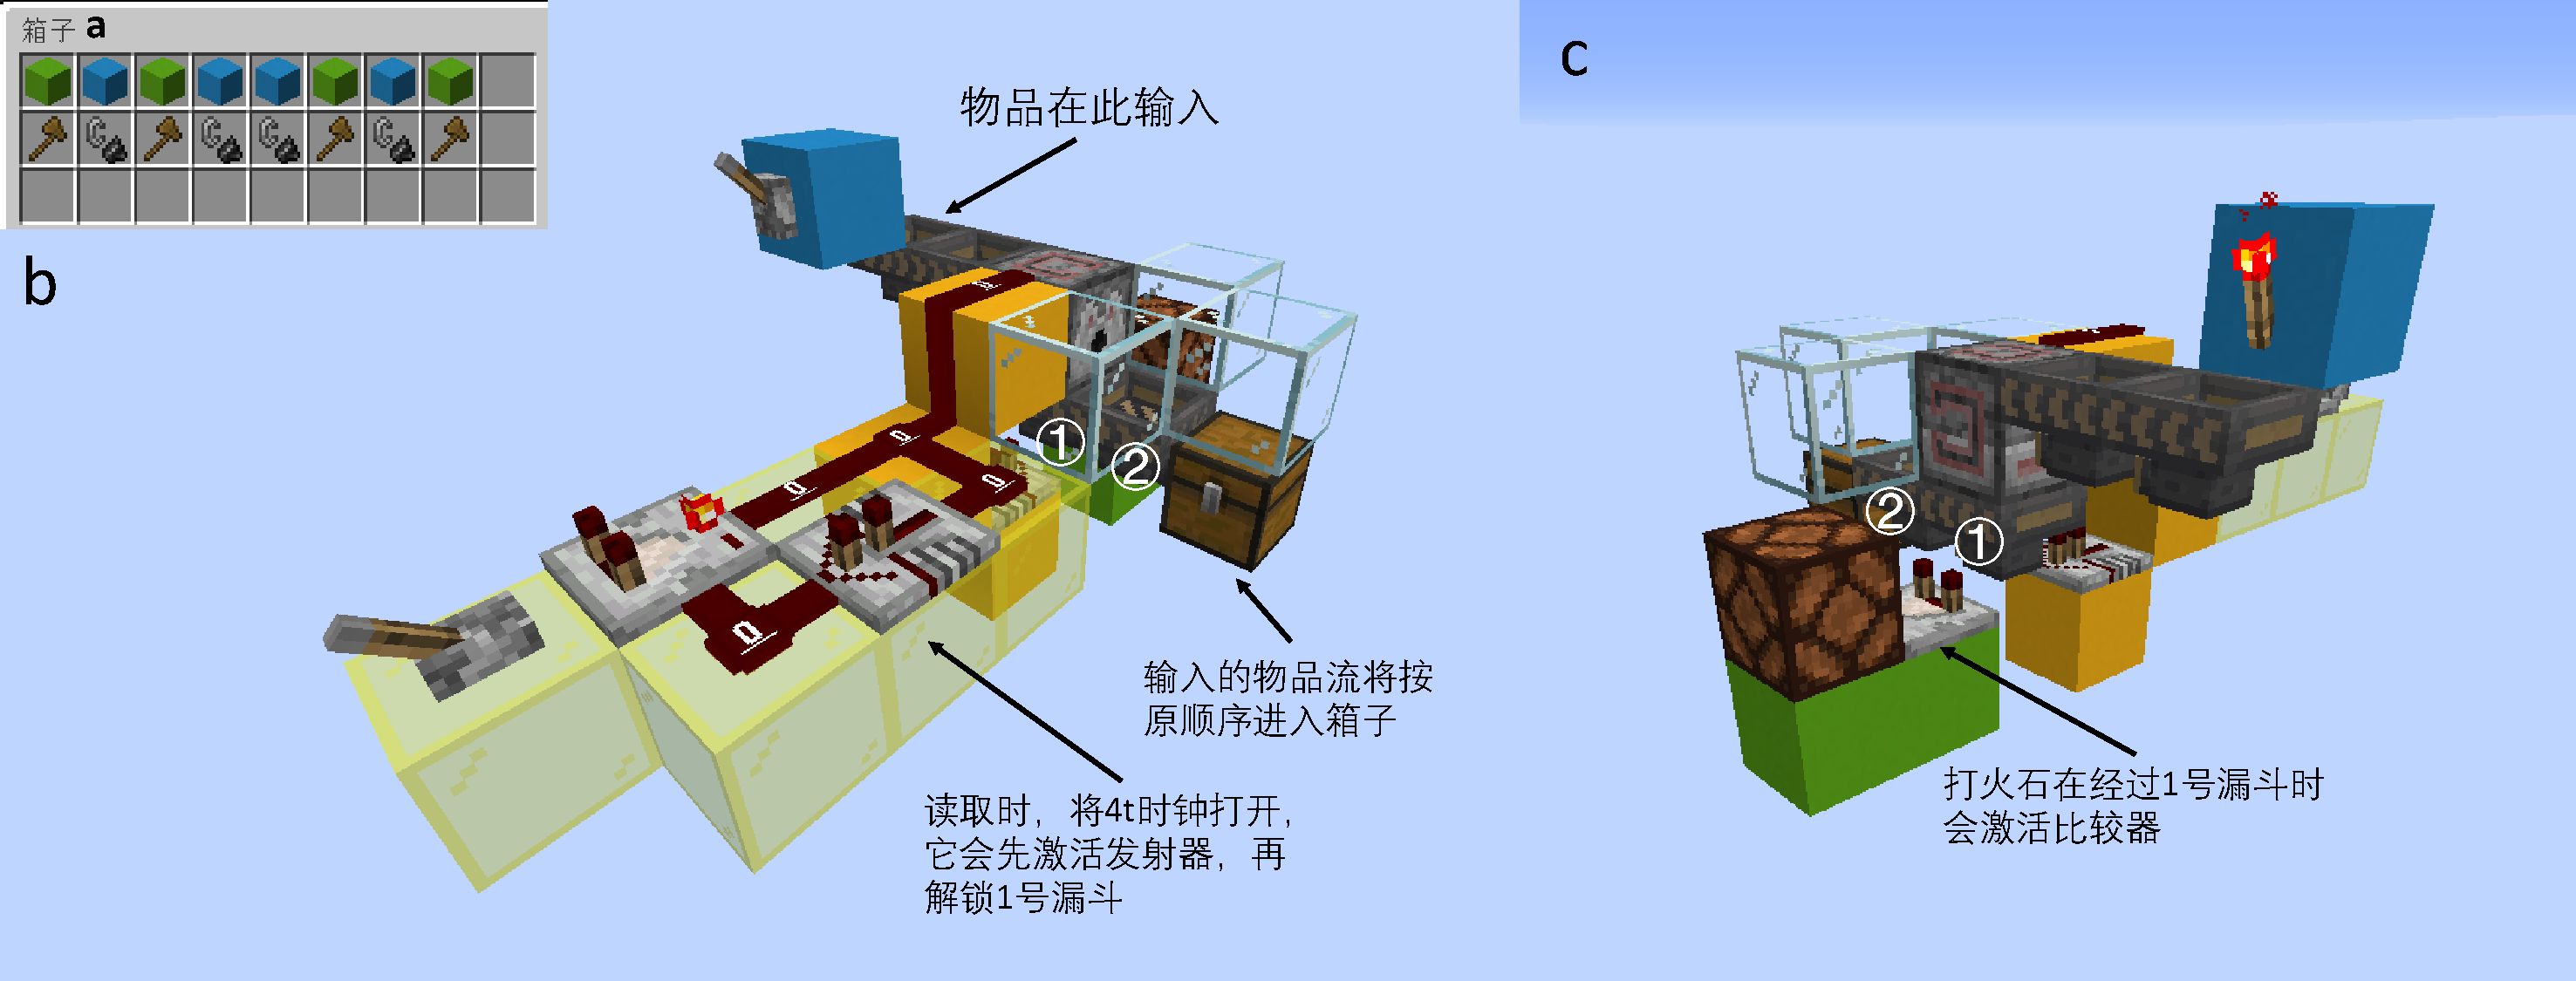
\includegraphics[width=.9\textwidth]{Fig1.pdf}
    \caption{(a) 编码方式。第一行为可堆叠物品,第二行为不可堆叠物品,打火石和木斧。
    (b)(c) 读取机器的样板机因为漏斗传输物品速度为4tick一个物品,所以匹配4tick时钟。时钟先激活发射器,后解锁漏斗。
    读取完毕后,输入的物品流按原顺序的进入箱子。}
    \label{fig:fig}
\end{figure}

%\bibliographystyle{unsrt}
%\bibliography{reference.bib}

\end{document}

